\subsection{Manifolds}

A manifold $\mathcal{M}$ is a shape which looks like a 'flat plane' from the perspective of a creature standing on it. This means that at every neighbourhood on this manifold there exists a homeomorphism (a continuous function whose inverse is also continuous) from the neighbourhood to a subset of $\mathbb{R}^n$ for some $n$. This $n$ is the dimension of the manifold. An easy example to wrap one's head around is a sphere, which is a two dimensional manifold. 

More specifically, at every point $p \in \mathcal{M}$ there exists an open set $\mathcal{P} $ with a homeomorphism $\phi_p : \mathcal{ P } \rightarrow U \subset \mathbb{R}^n $. These maps are called coordinate charts, and our collection of open sets $\mathcal{ P}_i $ should cover the manifold. 
\begin{figure}[h]
	\centering 
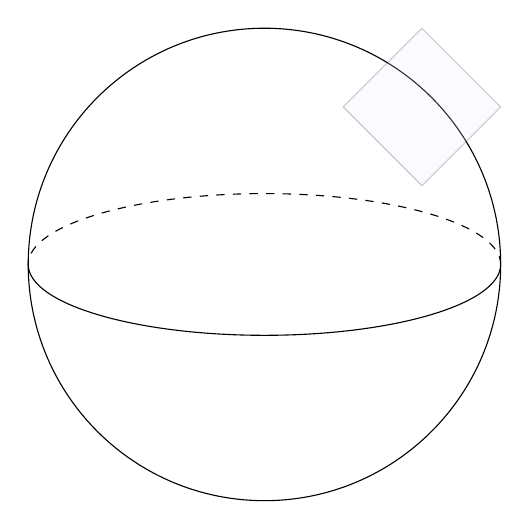
\begin{tikzpicture}
	\draw (0, 0) circle (3cm);
	\draw (-3, 0) arc (180:360:3 and 0.9);
	\draw[dashed] (3, 0) arc (0:180:3 and 0.9);

	\filldraw[fill=blue!10, opacity=0.2] (1, 2) -- (2, 3) -- (3, 2) -- (2, 1) -- cycle;  
   
\end{tikzpicture}
	\caption{A sphere locally looks like a flat plane, at any given point on the surface} 
\end{figure}

Since these homeomorphisms are from the manifold to $\mathbb{R}^n$, we can identify coordinates on an open set $\mathcal{P} \subset \mathcal{M}$, denoted by $\{ \theta^i \}$, where $i$ ranges from $i  = 1, 2, \dots, n$, where $n$ is the dimension of the manifold.

